\section{The remove command}

\subsection{How it works}
\textcolor{blue}{\textbf{remove}}: remove a file or directory at the provided path.\\

As we did in the read function we should also check here whether the path is correct or not. To do so, we can call the functions \textit{find\_file\_from\_path} and \textit{find\_dir\_from\_path}.\\

If the path is valid (i.e. there is something at this path in the file system), then we must get a non -1 value (-1 means the file/dir doesn't exist at this path). Else, if we get return value -1 for both of these functions, the path is not valid.\\

Now that we know whether the path refers to a file or a directory, we just need to call the adapted function to remove it (either \textit{rm\_directory or rm\_file)}. Those functions are file system functions, because they are used in other commands as well.\\

Removing a file is different from removing a directory.
On one hand, removing a file consists of removing the file from the \textit{file\_array} and then shift every other file to fill the gap.
On the other hand, removing a directory consists only of setting up the directory's \textit{parent\_id} to -1 (convention) and name to \textit{TRASHED}.\\

Directories should not be shifted like files, because we need to preserve the parent-child relationship between directories and this information is stored inside in \textit{parent\_id} member and their indices in the \textit{directory\_array}.\\

\begin{center}
    \begin{tabular}{cc}
        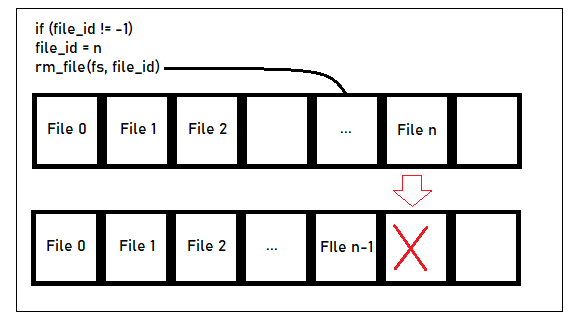
\includegraphics{figures/rm_file.png}
    \end{tabular}
    \captionof{figure}{Removing a file (made with MS Paint)}
\end{center}\\

\begin{center}
    \begin{tabular}{cc}
            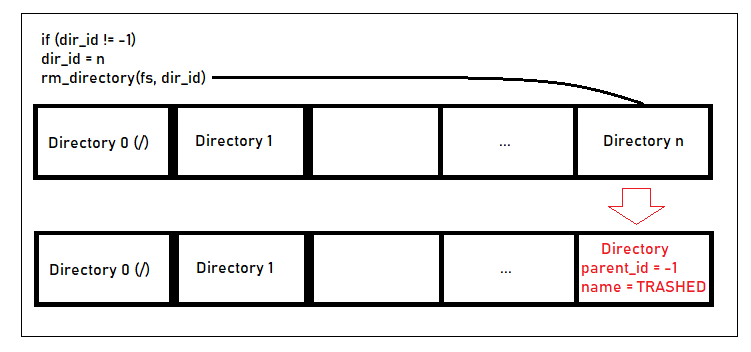
\includegraphics[width=16cm]{figures/rm_directory.png}
    \end{tabular}
    \captionof{figure}{Removing a directory (made with MS Paint)}
\end{center}\\

\newpage
\subsection{Testing}
\lstset{language=bash,caption={Remove command},label=code:remove-command}
\begin{lstlisting}
$ vmhFS /tmp/tmpFS write /tmp/foo.txt /dir1/dir2/foo.txt
$ vmhFS /tmp/tmpFS remove /dir1/dir2/foo.txt
$ vmhFS /tmp/tmpFS remove /dir1/dir2
$ vmhFS /tmp/tmpFS remove /dir1
$ vmhFS /tmp/tmpFS ls / -r
$ vmhFS /tmp/tmpFS remove /
\end{lstlisting}

\lstset{language=bash,caption={Command output},label=code:command-output}
\begin{lstlisting}
Write file /tmp/foo.txt to filesystem at: /dir1/dir2/foo.txt
File /dir1/dir2/foo.txt has been remove from the file system
Directory /dir1/dir2 has been remove from the file system
Directory /dir1 has been remove from the file system
List segment:
/
Root directory cannot be removed
\end{lstlisting}

\newpage
